\subsection{Training a global feature extractor}

\label{sec:modality_transfer}


\begin{frame}{CNN training}
	We begin with a pre-trained network and perform a \textbf{fine tuning} of its weights.
	\begin{block}{Encoder training for VBL task}
		\begin{figure}[c]
			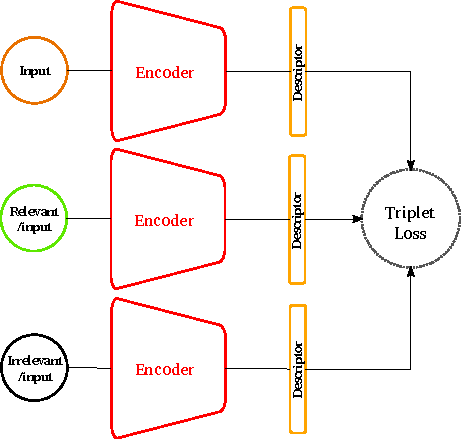
\includegraphics[width=0.5\linewidth]{vect/encoder_training.pdf}					
		\end{figure}
	\end{block}
\end{frame}

\begin{frame}{CNN training}
	
	\begin{block}{Training data}
		Triplet := (Query Image,  Positive example, Negative example)
		
		\hspace{1.8cm}
		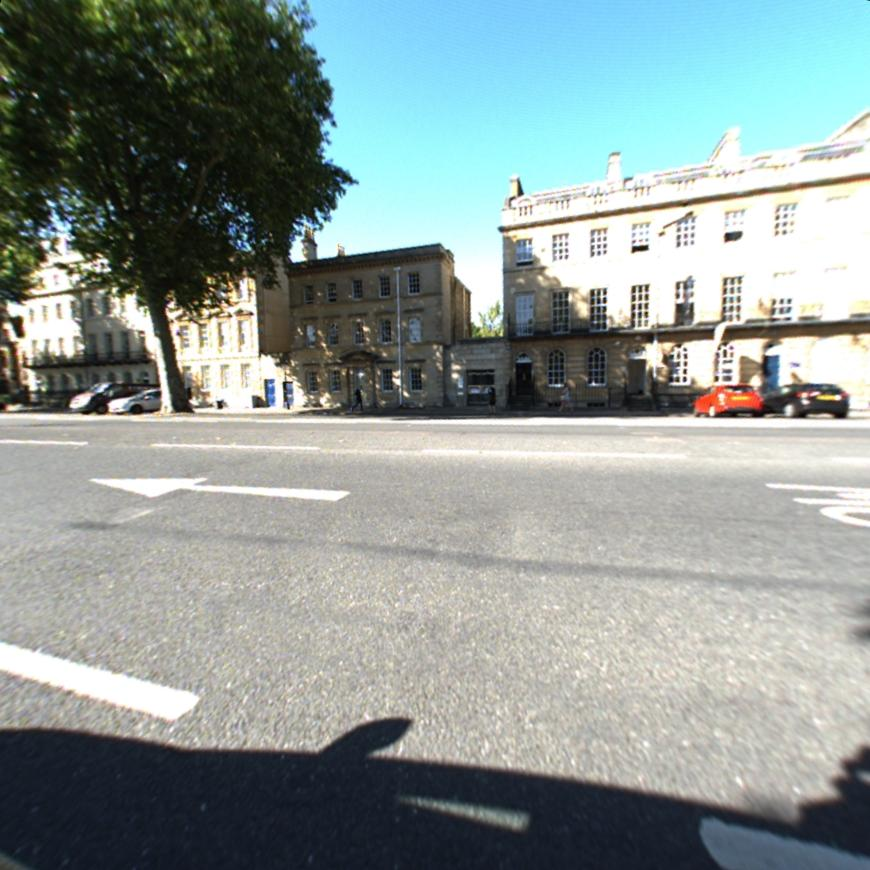
\includegraphics[width=0.2\linewidth]{images/query.jpg}\hspace{0.1cm}
		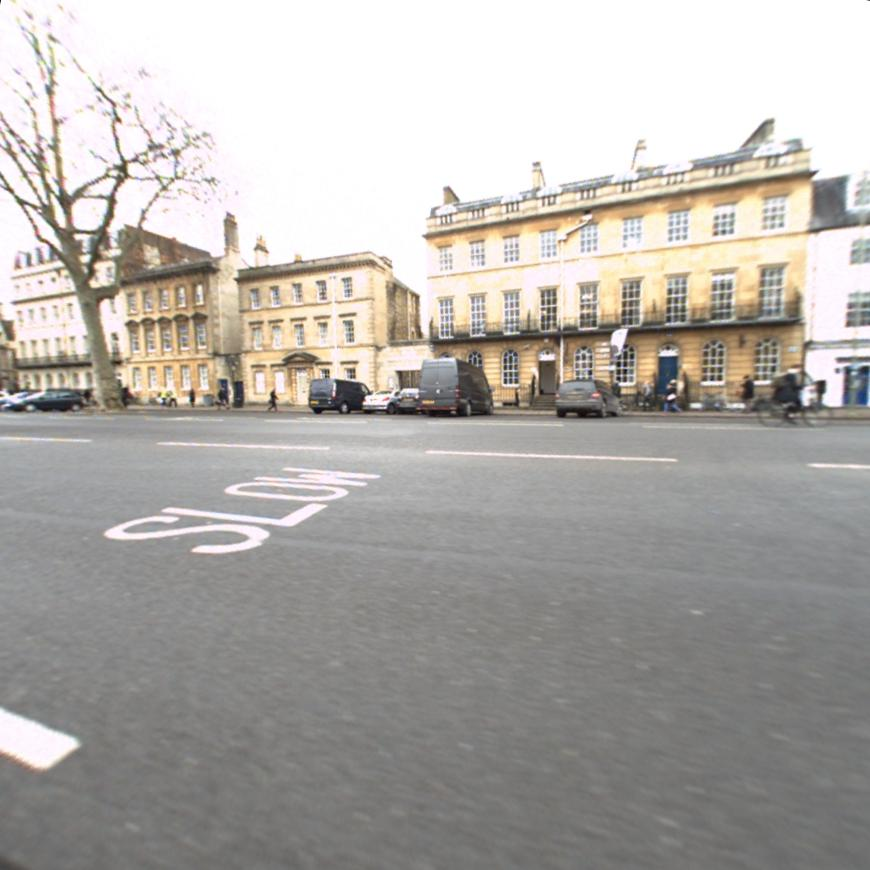
\includegraphics[width=0.2\linewidth]{images/positive.jpg}\hspace{0.1cm}	
		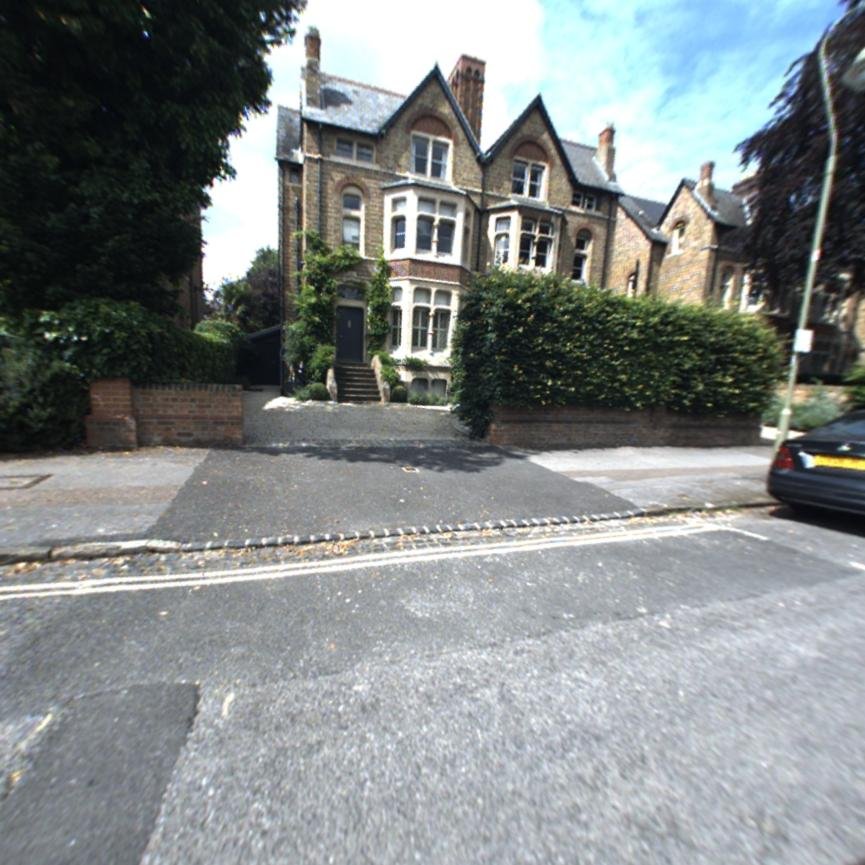
\includegraphics[width=0.2\linewidth]{images/negative.jpg}
		
	\end{block}
	
	\begin{block}{Cost function}
		During the training, we minimize the following loss:
		\begin{equation}
			TripletLoss = max(0, \lambda + \Vert F(I) - F(I^+) \Vert - \Vert F(I) - F(I^-) \Vert)
		\end{equation}
		Where:
		\begin{itemize}
			\item $F(I)$ the global descriptor of image $I$ computed by the CNN
			\item $\lambda$ design a constant margin
		\end{itemize}
	\end{block}

\end{frame}


\begin{frame}{Multiple modalities}
	How to use more than one modality at the time?
	\vfill
	\begin{block}{What are we first trying to do}
		\centering
		\begin{tabular}{c | c}
			\textbf{Training data type} & \textbf{Testing data type} \\
			\hline
			RGB + (Depth or Laser reflectance)  & RGB  \\
		\end{tabular}
	\end{block}
	\vfill
	We suppose that complex data (image + lidar related modality) can be acquired \textbf{offline}, but all the modality could not be available during test time. The idea is to guide the CNN during the training with \textbf{multiple modalities} to improve the description of input of \textbf{single modality}.
\end{frame}


\begin{frame}{Proposed architecture}	
	\begin{minipage}[c]{0.48\linewidth}
		\begin{block}{Encoder-Decoder architecture}
			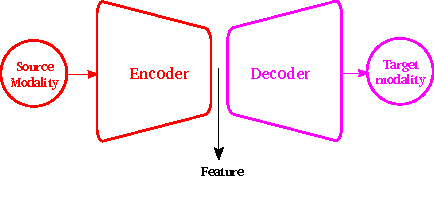
\includegraphics[width=\linewidth]{vect/encoderdecoder.pdf}					
		\end{block}
	\end{minipage}
	\hfill
	\begin{minipage}[c]{0.48\linewidth}
		\begin{block}{Encoder-Decoder training scheme}
			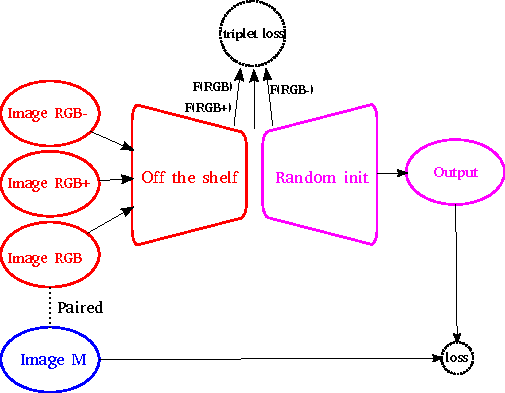
\includegraphics[width=\linewidth]{vect/encoderdecoder_training.pdf}	
		\end{block}
	\end{minipage}
	\vfill
	Decoder part is initialized with \textbf{pre-trained weights} and decoder network is randomly initialized.				
\end{frame}

\begin{frame}{Training}
	\begin{block}{Training data}
		Triplet := (Query Image + Modality,  Positive example, Negative example)
		
		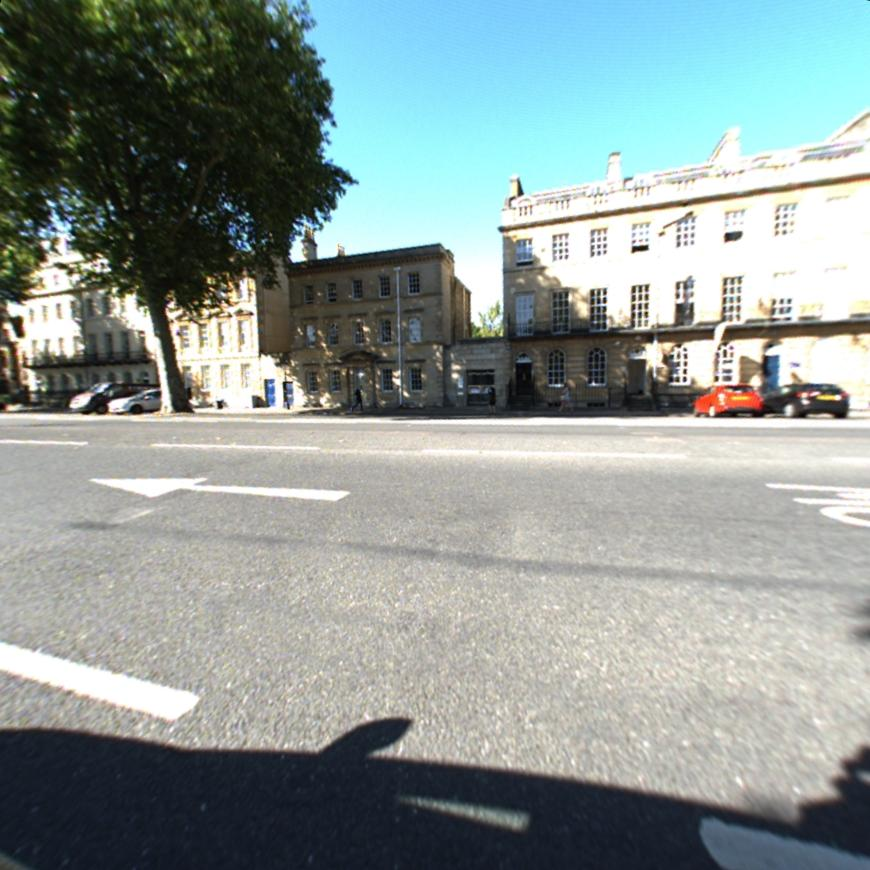
\includegraphics[width=0.2\linewidth]{images/query.jpg}\hspace{0.1cm}
		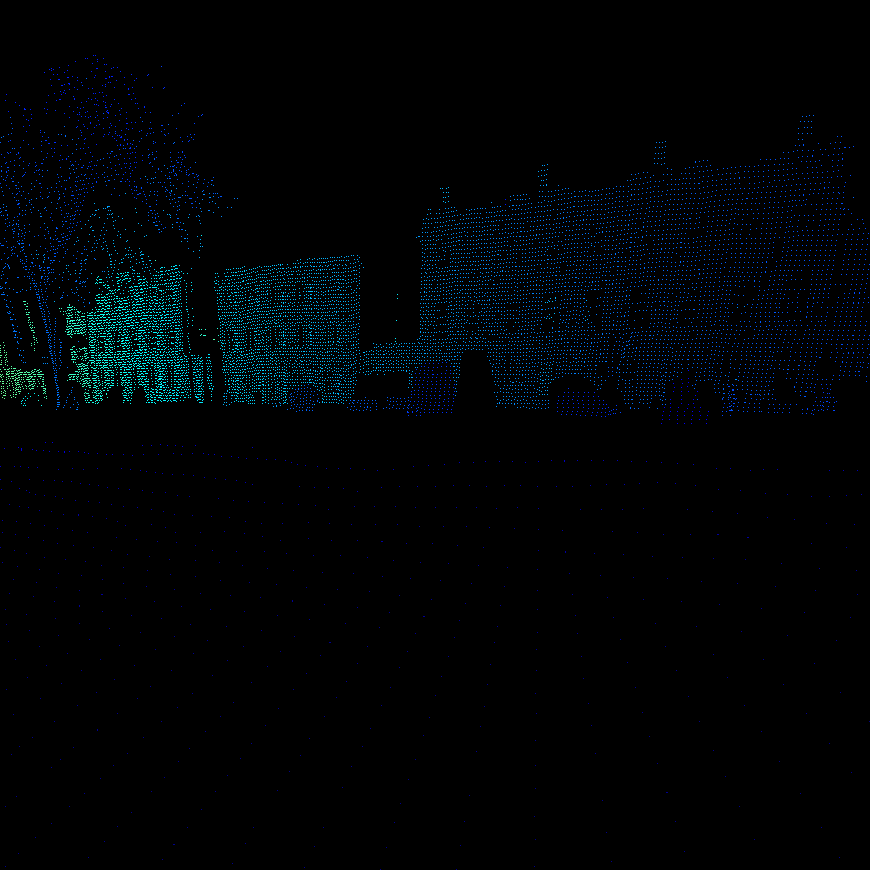
\includegraphics[width=0.2\linewidth]{images/qmodality.png}\hspace{0.1cm}
		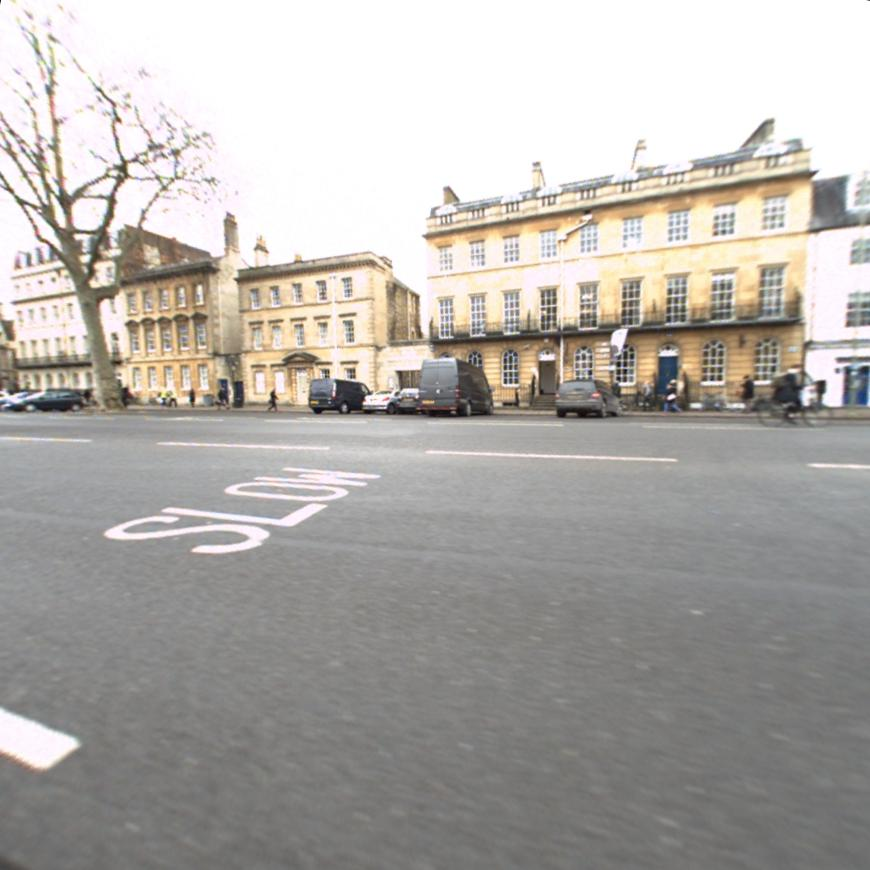
\includegraphics[width=0.2\linewidth]{images/positive.jpg}\hspace{0.1cm}	
		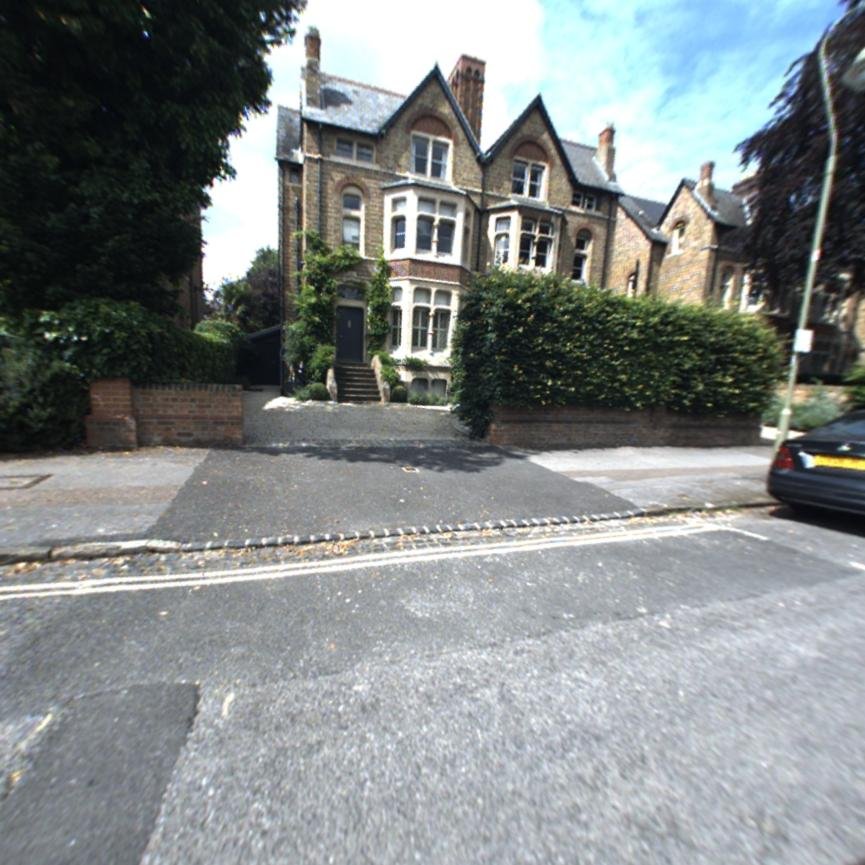
\includegraphics[width=0.2\linewidth]{images/negative.jpg}
	\end{block}
	
	\begin{block}{Cost function}
		Loss become \textbf{multi-task}:
		\begin{equation}
			L = TripletLoss +  \alpha\sum\limits_{i,j}^{h,w} |p(i,j)-gt(i,j)|
		\end{equation}
		Where:
		\begin{itemize}
			\item $p$ denote CNN inferred modality and $gt$ ground through modality
			\item $\alpha$ design loss weighting factor
		\end{itemize}
	\end{block}
\end{frame}

\begin{frame}{Datasets}	
	We use Oxford RobotCar dataset \cite{Maddern2016} as it includes:
	\begin{itemize}
		\item Time redundancy for each car trajectory and GPS tags associated to images: \textbf{automatic triplets creation!}
		\item 4 cameras on the car \& 3 LIDARS (3 modalities: RGB, Depth \& Reflectance)
	\end{itemize}
	\vfill
	\begin{minipage}[c]{0.22\linewidth}
		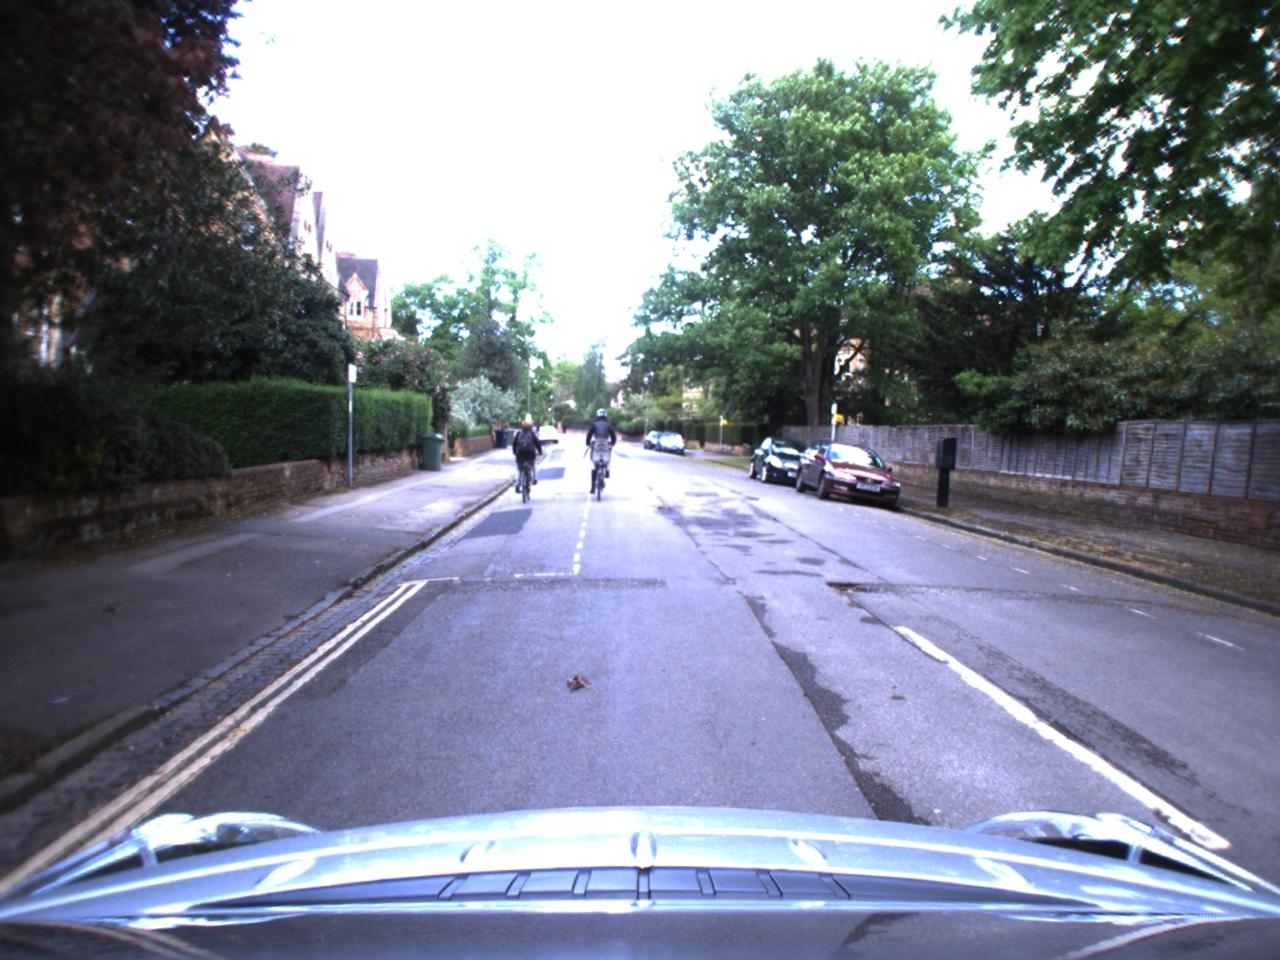
\includegraphics[width=\linewidth]{images/robotcar_1.jpg}
		
		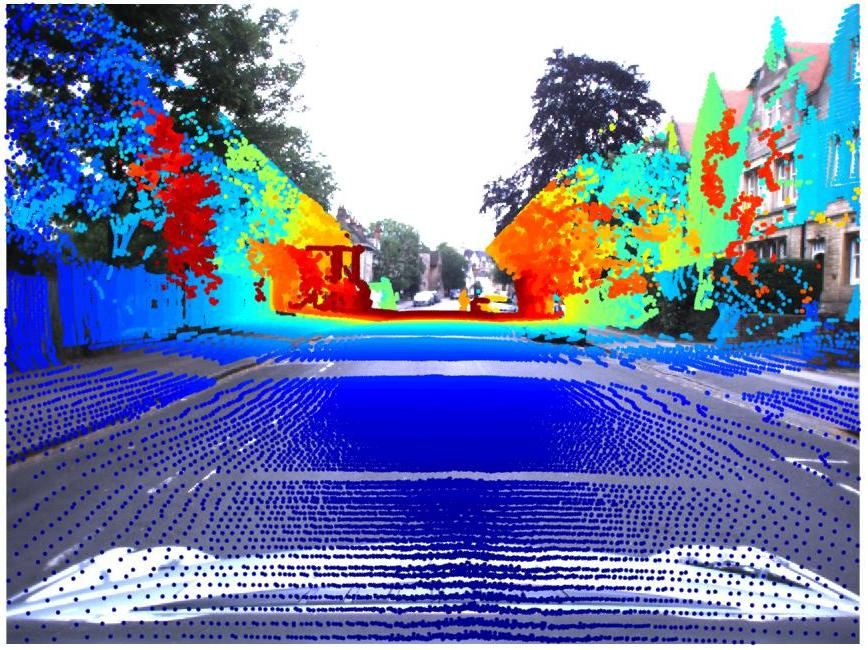
\includegraphics[width=\linewidth]{images/robotcar_depth.jpg}	
	\end{minipage}
	\hfill					
	\begin{minipage}[c]{0.77\linewidth}
		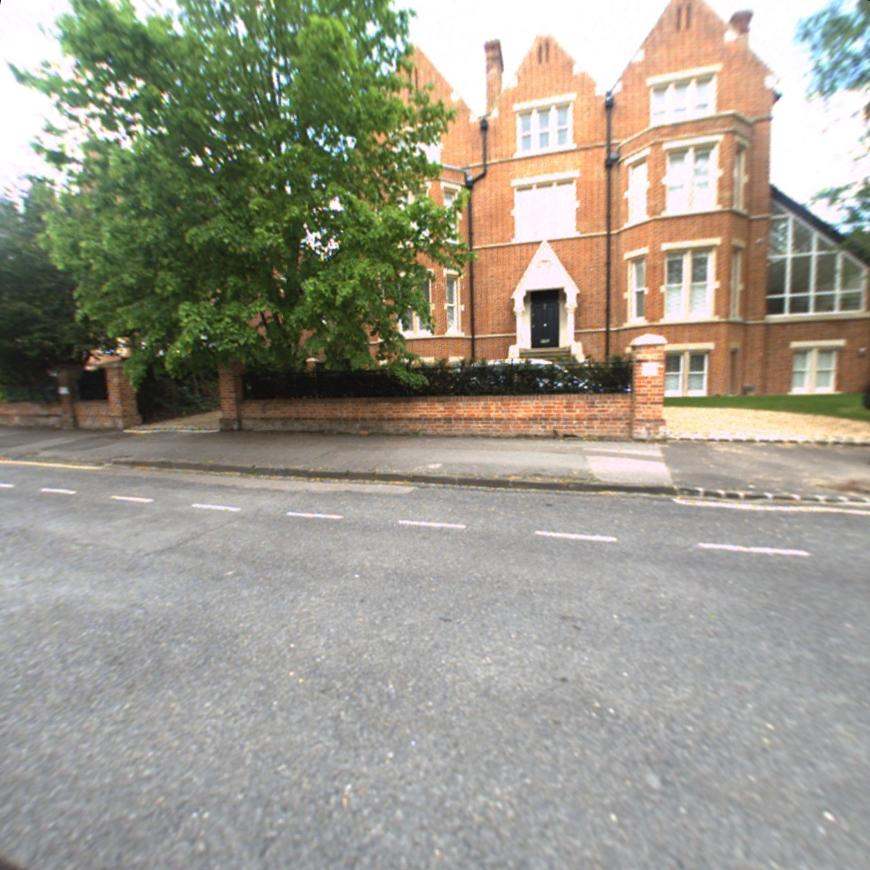
\includegraphics[width=0.3\linewidth]{images/robotcar_2.jpg}\hfill					
		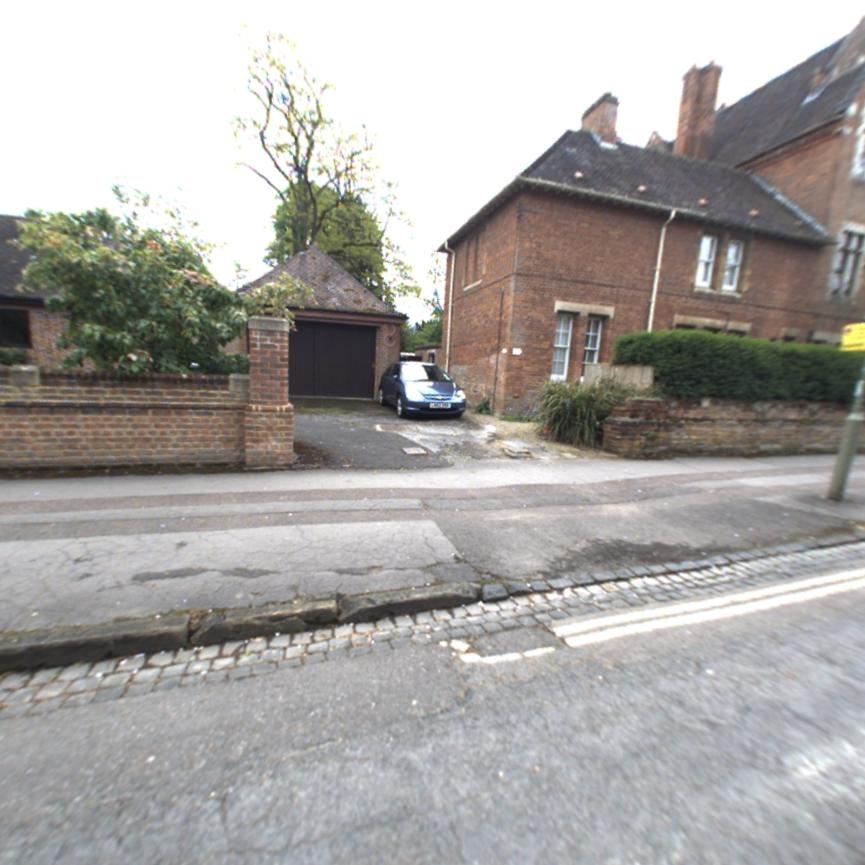
\includegraphics[width=0.3\linewidth]{images/robotcar_3.jpg}\hfill					
		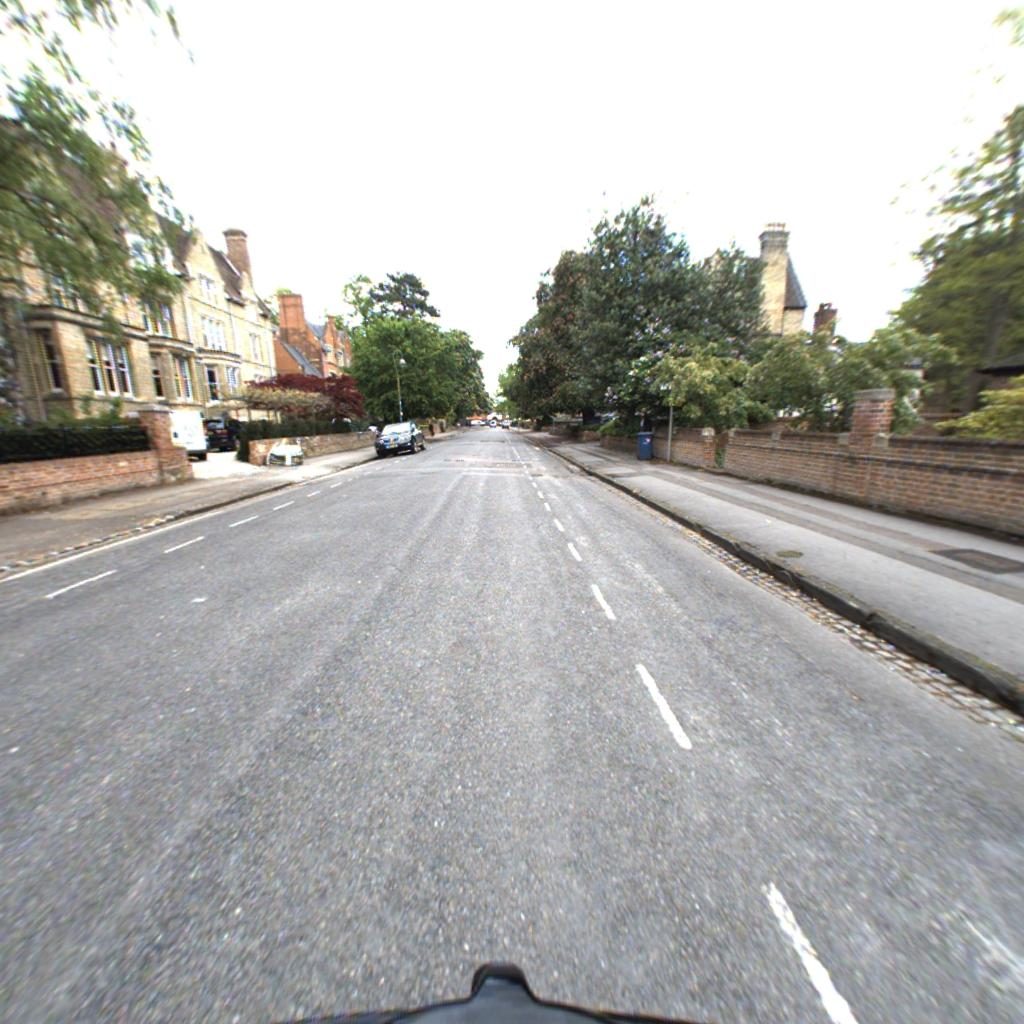
\includegraphics[width=0.3\linewidth]{images/robotcar_4.jpg}					
	\end{minipage}
\end{frame}

\begin{frame}{Important parameters for training}

	\begin{block}{Vocabulary}
        \begin{itemize}
        	\item \textbf{Forward pass:} operation to obtain input representation/classification
        	\item \textbf{Batch} several training example forward passed to a CNN before gradient computation and back-propagation
        	\item \textbf{Number of Epoch} correspond to the number of times all the batch data have been passed through the CNN
        	\item \textbf{Learning rate, Momentum, Weight decay, etc.} Meta-parameters of the optimizer used during the training
        \end{itemize}
	\end{block}	
	\vfill
	Hard and time consuming to fined all the best parameters...
\end{frame}